\documentclass[a4paper,twoside,12pt]{report}

% Load packages
% \usepackage[utf8x]{inputenc}
\usepackage[UKenglish]{babel}
\usepackage[round]{natbib}             % commands \citep e \citet for natural citations
\usepackage{nextpage}                  % blank pages with \cleartooddpage
\usepackage{amssymb}                   % maths stuff
\usepackage{amsfonts}                  % maths stuff
\usepackage{amsmath}                   % maths stuff
\usepackage{amsbsy}                    % maths stuff
\usepackage{color}                     % for coloured text & links
\usepackage{array,arydshln}
\usepackage{booktabs}                  % hrule with different widths and thicknesses
\usepackage{multirow}
\usepackage{pifont}
\usepackage{textcomp}
\usepackage{algpseudocode}             % for the algorithm pseudocode
\usepackage{setspace}                  % command \setstretch for line spacing on the text only
\usepackage[figuresright]{rotating}    % environment sidewaystable

% Temporary packages for testing
% \usepackage{graphicx}              % comment this out with XeLaTeX, but keep with pdfLaTeX
% \usepackage{lipsum}                % Lorem ipsum

% Use XeLaTeX and set fonts
\usepackage{mathspec}           % keep math standard TeX fonts, not XeTeX fonts
\usepackage{xltxtra}            % for the XeLaTeX stuff (it incorporates fontspec)
\defaultfontfeatures{Mapping=tex-text,Contextuals=Swash,Ligatures={Required,Common,Contextual,Rare}}
\setmainfont[Numbers=Lining]{Linux Libertine O}
\setromanfont[Numbers=Lining]{Linux Libertine O}
\setsansfont{Linux Biolinum O}
\setmonofont[Scale=MatchLowercase]{Linux Mono O}
\renewcommand{\thepage}{\arabic{page}} % font for the page numbers as lining

% Format for the captions
\usepackage[labelfont=bf,font=small]{caption}
% \usepackage[bf,small,sf]{caption}

% Some colors
\definecolor{corlink}{rgb}{0, 0, .4}
\definecolor{orange}{rgb}{.7, .40, 0}

% Hyperlinks setup and meta-information
\usepackage{hyperref}
\hypersetup{
  colorlinks,
  citecolor   = corlink,
  filecolor   = corlink,
  linkcolor   = corlink,
  urlcolor    = corlink,
  pdftitle    = {New Strategies for Permutation Methods in Brain Imaging},
  pdfauthor   = {Anderson M. Winkler}}

% Header and footer
\usepackage{fancyhdr}
\usepackage[fit]{truncate}
\fancyhead[RE]{\truncate{0.9\headwidth}{\small\nouppercase{\textbf{\leftmark}}}}
\fancyhead[LO]{\truncate{0.9\headwidth}{\small\nouppercase{\textbf{\rightmark}}}}
\fancyhead[RO,LE]{\small\arabic{page}}  % right odd, left even
\fancyfoot{}
% \fancyfoot[C]{\textcolor{red}{\textbf{--- UNCORRECTED PROOF ---}}}

% Margins (this uses fancyhdr package)
%\usepackage{showframe}
\topmargin      = 0mm
\oddsidemargin  = 16mm % 5mm
\evensidemargin = 4mm  % 5mm
\marginparsep   = 0mm
\marginparwidth = 0mm
\textwidth      = 140mm
\textheight     = 225mm
\headwidth      = 140mm
\headheight     = 6mm

% Adjust footnotes indentation
\usepackage[hang,flushmargin]{footmisc} 
\renewcommand{\footnotemargin}{.8em}

% Other new commands
\newcommand{\ud}{\mathrm{d}}
\newcommand{\blankpage}{\cleartooddpage[\thispagestyle{empty}]}
\newcommand{\HRule}{\rule{\linewidth}{0.08em}}
\renewcommand\multirowsetup{\centering}

% Line spacing
%\linespread{1.35} % this affects everything
\newcommand{\lspac}{1.5}  % this affects only the main text, not footnotes, captions or tables
\setlength{\skip\footins}{10mm} % distance between text and footnotes
\setlength{\footnotesep}{4mm} % distance between the actual footnotes

% Sections up to level 4
\setcounter{secnumdepth}{3}
\setcounter{tocdepth}{3}

% For the title page
\title{New Strategies for Permutation\\Methods in Brain Imaging}
\author{Anderson M. Winkler}

\begin{document}
\maketitle
\bibliographystyle{latex/scabbrvnat}

\pagestyle{fancy}
\setstretch{\lspac}
\blankpage \tableofcontents
\blankpage \listoffigures
\blankpage \listoftables
% \blankpage \listofalgorithms
\setstretch{1}
\blankpage \chapter{Introduction}
\setstretch{\lspac}

It has been suggested that the processes that drive horizontal (tangential) and vertical (radial) development of the cerebral cortex are separate from each other \citep{Rakic1988}. Variations on these would result, respectively, in variations on the extent of cortical surface area and on the thickness of the cortical mantle. Through the use of genetically informative samples, it has been demonstrated these two processes are indeed uncorrelated genetically \citep{Panizzon2009, Winkler2010} and are each influenced by regionally distinct genetic factors \citep{Schmitt2008,Rimol2010a}. Moreover, it is variation on surface area that explains most of the variation observed in the amount of gray matter assessed with methods that only measure volume, such as voxel-based morphometry \citep{Winkler2010, Rimol2012}.

These findings give prominence to the use of surface area alongside cortical thickness in studies of brain morphology and, and its interaction with brain function. However, cortical surface area been measured only over gross regions or approached indirectly via comparisons with a standard brain. Of studies using the latter, few that have used area measurements on every point of the cortex (vertexwise) and have offered detailed insight on the exact procedures used for this assessment. Some studies described their methods in terms of ``expansion/contraction'', often using different definitions of what expansion or contraction would be. By 2011, various impromptu approaches had been considered, for example:

\begin{itemize}
\item[--] \citet{Lyttelton2009}: The authors describe that the asymmetry measurement is the logarithm of the ratio of the area per vertex of left and right hemispheres. Expansion or contraction are in relation to the contralateral hemisphere.
\item[--] \citet{Joyner2009}: After a brief description of the method of measurement, the authors state that ``(\ldots) this provides point-by-point estimates of the relative areal expansion or compression of each location in atlas space.'' Expansion/contraction are relative to the chosen template.
\item[--] \citet{Sun2009a}: The authors state that ``The distance between a center position of the brain (\ldots) and each brain surface point was calculated (\ldots). The difference of the above radial distances between the follow-up and baseline brain surfaces (\ldots) was defined as brain surface contraction''. Under this definition, not only contraction refers to an initial point in time, but it also refers not to a bidimensional feature, and instead to a linear distance between each point in the surface and a given central point in the brain.
\item[--] \citet{Sun2009}: The authors state that ``The distance between two brain surfaces [\emph{i.e. inner skull and pial}] was then measured at subvoxel resolution (\ldots), the value in millimeters was assigned to the voxel as the intensity value and an image of the brain surface contraction was obtained''. Under this definition, for a longitudinal study, the contraction is the difference between initial and final distances between inner skull and pial surfaces, assigned to a volumetric (voxel-based) space.
\item[--] \citet{Hill2010}: The article discusses growth of the cortex from birth to adulthood and compares it with the cortex of the monkey. Here expansion can be interpreted as in relation to an initial, developmental and/or evolutionary stage, not to a given template or to the other hemisphere.
\item[--] \citet{Rimol2010b}: Expansion and contraction are measured in relation to a template, as in \citet{Joyner2009}.
\item[--] \citet{Palaniyappan2011}: The authors state that ``In line with \citet{Joyner2009}, we use the term contraction to suggest group differences in the surface area in patients compared to controls, rather than a reduction from previously larger area.'' This in fact seems a new interpretation over the method used by \citet{Joyner2009}, as the authors here would then be using expansion/contraction to compare to the control group. Yet, reading through the article, it appears clear that expansion/contraction still refers to the chosen template.
\item[--] \citet{Chen2011_neuron,Chen2012}: The authors use a method similar to \citet{Joyner2009} and \citet{Rimol2010b}, and so, expansion/contraction refer to the template.
\end{itemize}

All these different operating definitions of what expansion/contraction would be create already difficulties in the interpretation of their meaning. However, even if only one of these existed, it would still be difficult to interpret, due to the dependence of all these methods on a reference brain or on the contra-lateral hemisphere, from which expansion or contraction is tentatively assessed.

In the present work, we propose a method that uses absolute quantities, as opposed to being relative to a reference brain. While initially addressing these concerns, we found yet others that required further investigation. The first is that we found that surface area is lognormally distributed, such that direct use of statistical methods based on the assumption of normality are likely to yield incorrect results. The second concerns use of data assigned to each face of a mesh representation of the brain, as opposed to each vertex, which cannot be analysed in software designed to handle vertexwise data, nor stored in vertexwise file formats, thus demanding the development of new tools for analysis and a file format. The third is that in neuroimaging thousands of tests are performed in an image representation of the brain. None of the parametric methods can be considered for control of the familywise error rate, given the lognormality and the spatial dependencies among the data assigned to each face of the mesh representation without appealing to many unrealistic assumptions, thus demanding the use of more flexible approaches.

Treating these problems eventually that led into a complete framework for the measurement and statistical analysis of areal quantities. It uses permutation tests in the general linear model, and yet allowing area and thickness to be studied jointly without appealing to cortical volume. Nonetheless, the method can also be used to study volume, either using the current approach of multiplying cortical area by cortical thickness, or else, using an improved method that we propose, in which no pieces of the cortex are left over- or under-represented.

Although this work can be organised into three core topics that are relatively independent from each other, and that have each been published as separate papers \citep{Winkler2012, Winkler2014, Winkler2016}, the flow of information in a complete study of cortical morphology visits all three, as shown in Figure~\ref{fig:intro:flow}. The next sections outline these three main chapters. Each chapter offers a detailed introduction describing the problem that each aim to solve, along with review of the relevant literature, evaluation and implementation, including algorithms as needed, and a detailed discussion.

\begin{figure}[tbp]
\begin{center}
\centerline{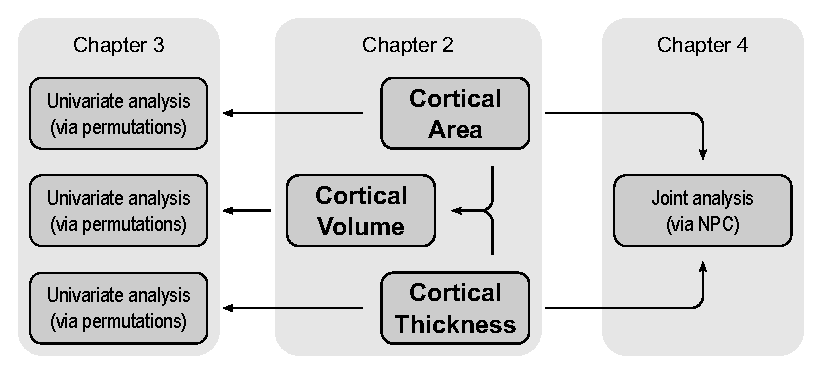
\includegraphics{images/flow.eps}}
\end{center}
\caption[Some possible analyses of cortical morphometric measurements using permutation tests.]{Some possible analyses of cortical morphometric measurements using permutation tests. Inter-subject comparisons of cortical area and other areal quantities, such as volume, that depends on both area and thickness, use the methods proposed in Chapter~\ref{sec:areal}. Univariate statistical analysis of each of these separately use the strategy discussed in Chapter~\ref{sec:perm}. Joint (combined) analysis of area and thickness, that bypass volumes altogether, use the methods proposed in Chapter~\ref{sec:comb}, in particular the non-parametric combination (\textsc{npc}), but also classical multivariate tests.}
\label{fig:intro:flow}
\end{figure}

\section{Methods for areal quantities}

The general strategy for analyses of cortical measurements consists of the generation of a surface-representation of the brain and its subsequent transformation into a sphere. Vertices of this sphere are then shifted along its surface to allow alignment that matches some feature of interest, such as sulcal depth, myelin content, or functional markers. As the alignment is performed, quantities assigned to vertices or faces, such as thickness or area, are carried along these vertices and faces. Once registration is done, these quantities are interpolated to a common grid (mesh), where comparisons between subjects can be performed.  

While methods to study thickness across subjects are available \citep{Fischl2000}, and use interpolation to a common reference grid using methods such as nearest neighbour or barycentric, such interpolation strategies cannot be used for either cortical area itself, nor to other areal quantities, such as cortical volume, as these are not mass-conservative (pycnophylactic). Chapter~\ref{sec:areal} clarifies the distinction between the nature of these measurements, and proposes the use of areal interpolation. This strategy permits quantities to be studied in absolute terms, as opposed to relative to some reference brain. The chapter proposes that areal quantities are analysed directly in the faces of the mesh from which they were computed, instead of resampled to vertices, which halves the resolution.

We demonstrate that areal data do not follow a normal distribution, being better characterised by a mixture of normal and lognormal distributions, in proportions that vary across the brain and possibly according to the scale of measurement. A power transformation can be considered to address lognormality, although a better alternative is to use permutation methods, that not only do not rely on distributional assumptions, but also allow correction for multiple testing and the use of non-standard statistics.

\section{Methods for permutation inference}

Permutation methods can provide exact control of false positives, making only weak assumptions about the data, and have been available in brain imaging for many particular cases \citep{Holmes1996, Nichols2002}, although no implementation for surface-based methods, even less so for facewise data as we have developed, existed in the literature until this work. With the recent availability of fast and inexpensive computing, the main limitation of permutation tests would be a certain lack of flexibility with respect to arbitrary experimental designs, in particular with respect to nuisance variables in the model, as well as repeated measurements. 

In Chapter~\ref{sec:perm} we report on results on approximate permutation strategies that are more flexible with respect to experimental designs that include such nuisances. We review the literature and conduct detailed simulations to identify the best method for settings that are typical for imaging research. A generic framework for permutation inference for complex general linear models (\textsc{glm}s) when the errors are exchangeable and/or have a symmetric distribution, is presented. Even in the presence of nuisance effects, these permutation inferences are powerful and provide control of false positives in a wide range of common and relevant imaging research scenarios.

We also demonstrate how the inference on \textsc{glm} parameters, originally intended for independent data, can be used in certain special but useful cases in which independence is violated, by means of using exchangeability blocks, that is, sets of observations with shared non-independence, and that can sometimes be treated as a single unit for permutation, i.e., shuffled as a whole, or sometimes serve as delimiters such that permutations happen only within block. The definition of exchangeability blocks allow for groups of observations with same variances, either known or assumed, thus requiring a statistic that preserves certain desirable properties for control of multiple testing even under such scenarios. We provide such a statistic, dubbed $G$-statistic, which is a generalisation of the $F$-statistic, as well as others.

\section{Methods for joint permutation inference}

While gray matter volume can be studied directly using the methods discussed in Chapter~\ref{sec:areal}, it may be the case that true effects affecting thickness and area in opposite directions may cancel each other out. Yet, analysing them separately using univariate methods as in Chapter~\ref{sec:perm} may not aggregate power from having effects acting the two simultaneously. Likewise, participants of an imaging study are often subjected to the acquisition of more than one imaging modality. These modalities are often analysed separately. However, a joint analysis have potential to answer more complex questions and to increment power. Moreover, even a single modality can sometimes be partitioned into subcomponents that disentangle different aspects of brain structure or function. Examples include independent component analysis, as well as scalar measurements from diffusion-tensor imaging. 

In Chapter~\ref{sec:comb} we show how permutation methods can be applied to combination analyses such as those that include multiple imaging modalities, multiple data acquisitions of the same modality, or simply multiple hypotheses on the same data. Using the well-known definition of union-intersection tests and closed testing procedures, we use synchronised permutations to correct for such multiplicity of tests, allowing flexibility to integrate imaging data with different spatial resolutions, surface and/or volume-based representations of the brain, including non-imaging data. 

In particular for the problem of joint inference, we propose and evaluate a modification of the recently introduced Non-Parametric Combination (\textsc{npc}) methodology \citep{Pesarin2010}, such that instead of a two-phase algorithm and large data storage requirements, the inference can be performed in a single phase, with reasonable computational demands. We also evaluate, in the context of permutation tests, various combining methods that have been proposed in the past decades, and identify those that provide the best control over error rate and power across a range of situations. We show that one of these, the method of \citet{Tippett1931}, provides a link between correction for the multiplicity of tests and their combination.

Finally, we discuss how the correction can solve certain problems of multiple comparisons in common designs, and how the combination is distinguished from conjunctions, even though both can be assessed using permutation tests. We also provide a common algorithm that accommodates combination and correction.
\blankpage \include{20facewise}
\blankpage \chapter{Piecewise volume}
\setstretch{\lspac}


\blankpage \include{40permutation}
\blankpage \chapter{Combination inference}
\label{sec:comb:combination}
\setstretch{\lspac}

\section{Introduction}

% IUT
% Conjunction/disjunction
% partial, marginal
% F-tests, rejection regions
% FWER 
% Meta-analysis
% Diagram, comparison
% Relationship with cognition, biological interpretation

% Implementation aspects: avoid being close to 1, etc
% Common framework for different tests

% Uses of NPC
% - Different modalities
% - Same modality, different aspects -- ICs, DTI scalars, thick/area
% - Repeated measurements
% - Non-orthogonal studies

% Philosophical questions: should we combine or dissect?

The previous chapter discussed how permutation methods, for being free of various assumptions related to classical parametric tests, could better adapt to the growing variety of experimental imaging methods. In this chapter, these ideas are further extended to non-parametrically allow \emph{joint inference} on more than one modality, that is, how to infer about hypotheses concerning these modalities when more than one image is available for each subject. Examples of such modalities include the same cited in Chapter~\ref{sec:comb:permglm}, such as, but not limited to, positron emission tomography (\textsc{pet}), functional magnetic resonance imaging (\textsc{fmri}), tensor-based morphometry (\textsc{tbm}), diffusion tensor imaging (\textsc{dti}), cortical thickness and surface area, cerebral perfusion, as well as various others.

Further to these examples, it is also the case that the same imaging modality is often subdivided so as to better characterise certain physical properties --- including morphology and function --- of the biological tissue. As an example, diffusion-weighted images are often used to generate maps of fractional anisotropy (\textsc{fa}), mean diffusivity (\textsc{md}), radial diffusivity (\textsc{rd}), as well as lengths of the eigenvectors of the diffusion tensor and other measurements. Another example is the use of independent component analysis (\textsc{ica}) to decompose \textsc{fmri} time series into a set of timecourses and spatial maps. Only some of these components might be of actual interest, or the effect of interest might be split into more than one; in either case, a strategy that could combine the information from these into a single inferential step tends to be more meaningful than various separate tests.

Historically, as in the case of the permutation tests discussed in Chapter~\ref{sec:comb:permglm}, Ronald A.\ Fisher was among the first to propose such joint analysis of various tests. In the fourth edition of his now classical book \textit{Statistical Methods for Research Workers} \citep{Fisher1932}, his approach was described rather succinctly:

\begin{quote}
\emph{When a number of quite independent tests of significance have been made, it sometimes happens that although few or none can be claimed individually as significant, yet the aggregate gives an impression that the probabilities are on the whole lower than would often have been obtained by chance. It is sometimes desired, taking account only of these probabilities, and not of the detailed composition of the data from which they are derived, which may be of very different kinds, to obtain a single test of the significance of the aggregate, based on the product of the probabilities individually observed.}

\emph{The circumstance that the sum of a number of values of $\chi^{2}$ is itself distributed in the $\chi^{2}$ distribution with the appropriate number of degrees of freedom, may be made the basis of such a test. For in the particular case when $n=2$, the natural logarithm of the probability is equal to $\frac{1}{2}\chi^{2}$. If therefore we take the natural logarithm of a probability, change its sign and double it, we have the equivalent value of $\chi^{2}$ for 2 degrees of freedom. Any number of such values may be added together, to give a composite test, using the Table of $\chi^{2}$ to examine the significance of the result. \hfill --- \citet{Fisher1932}}
\end{quote}

The logic of this test is based on the fact that the probability of rejecting the global null hypothesis is related to intersection of the probabilities of each individual test, i.e., $\prod_{i} P_{i}$. However, $\prod_{i} P_{i}$ is not uniformly distributed, even if the null is true for all partial tests, and cannot be used itself as the joint significance level for the global test. To remediate this fact, some interesting properties and relationships among distributions of random variables were exploited by Fisher and embodied in the succinct excerpt above:

\paragraph{The logarithm of uniform is exponential} The cumulative distribution function (cdf) of an exponential distribution is $F(x)=1- e^{-\lambda x}$ where $\lambda$ is the rate parameter, the only parameter of this distribution. The inverse cdf is, therefore, given by $x = -\dfrac{1}{\lambda}\ln(1-F(x))$. $F(x)=P$ is a random variable uniformly distributed in the interval $[0, 1]$, and so is $1-P$, and it is immaterial to differ between them. As a consequence, the same can be written as $x = -\dfrac{1}{\lambda}\ln(P)$, where $P \sim \mathcal{U}(0,1)$, which highlights the fact that the negative of the natural logarithm of a random variable distributed uniformly between 0 and 1 follows an exponential distribution with rate parameter $\lambda=1$.

\paragraph{An exponential with rate 1/2 is $\chi^2$ distributed} The cdf of a chi-squared distribution with $\nu$ degrees of freedom, i.e. $\chi^{2}_{\nu}$, is given by $F(x; \nu) = \dfrac{\int_{0}^{x/2} t^{\frac{\nu}{2}-1}e^{-t}{\rm d}t}{\left(\frac{\nu}{2}-1\right)!}$. If $\nu=2$, the expression simplifies to $F(x; \nu=2) = 1-e^{-x/2}$. In other words, a $\chi^{2}$ distribution with $\nu=2$ is equivalent to an exponential distribution with rate parameter $\lambda=1/2$.

\paragraph{The sum of chi-squared is also chi-squared} The moment-generating function (mgf) of a sum of independent variables is the product of the mgfs of the respective variables. The mgf of a $\chi^{2}_{\nu}$ is $M(t) = (1-2t)^{-\nu/2}$. The mgf of the sum of $K$ independent variables that follow each a $\chi^{2}_{2}$ distribution is then given by $M_{\text{sum}}(t) = \prod_{i=1}^{K} (1-2t)^{-2/2} = (1-2t)^{-K}$, which also defines a $\chi^{2}$ distribution, however with degrees of freedom $\nu=2K$.

With these facts in mind, the product $\prod_{i} P_{i}$ can be transformed into a p-value that is uniformly distributed when the global null is true. The product can be converted into a sum by taking the logarithm. And as shown above, the logarithm of uniformly distributed variables follows an exponential distribution with rate parameter $\lambda=1$. Multiplication of each $\ln(P_{i})$ by 2 changes the rate parameter to $\lambda=1/2$ and makes this distribution equivalent to a $\chi^{2}$ distribution with degrees of freedom $\nu=2$. The sum of $k$ of these logarithms also follow a $\chi^2$ distribution, now with $\nu=2K$ degrees of freedom, i.e., $\chi^{2}_{2K}$. Thus, the statistic for the Fisher method is given by $T_{\text{Fisher}}$ $=$ $-2 \sum_{i=1}^{K} \ln(P_{i})$, with $T_{\text{Fisher}}$ following a $\chi^{2}_{2K}$ distribution, from which a p-value for the global hypothesis can be easily obtained.

The elegance of the combination strategy devised by Fisher resides in that it depends solely on the uniformity of the distribution of the p-values for each of the separate $K$ tests under the null hypothesis, something that, by definition, is always attained whenever a statistical test is exact. This also renders the test, in a certain sense, non-parametric, although arguably, the number of tests can be considered a parameter upon which the resulting combined statistic depends.

\section{Parametric combination strategies}

The logic followed by Fisher is helpful to understand the behaviour of various other approaches. All of them pool a summary statistic from the original tests to produce a new, joint statistic. This joint statistic is used to assess significance of the aggregate of the tests. Consider $K$ independent tests, each with their respective p-values $p_{k}$, $k=\{1$, $\ldots$, $K\}$. These tests can also be called \emph{partial tests} \citep{Pesarin2010}, and each can, individually, be declared significant or not at certain level $\alpha$. For each combining method, an overall statistic $T_{\text{(method)}}$ is obtained, from which a p-value, $P_{\text{(method)}}$, is computed to reject or not, at a given significance level $\gamma$, the \emph{global null hypothesis}\footnote{Also called \emph{conjunction of null hypotheses} \citep{Benjamini2008}.} that there is no effect for all partial tests. Here the same significance level $\alpha$ is used for all of the partial tests, although some methods permit the use of a different $\alpha$ for each.

A list of these methods is presented below, in chronological order as they were published, and summarised in Table~\ref{tab:comparisonC}. All of these could be termed as ``non-parametric'' for not depending on the underlying distribution of the data for the original tests, only on their p-values, although most are still ``parametric'' in the sense that most have a known asymptotic distribution for their respective statistic $T_{\text{(method)}}$ if certain assumptions are met for each case. As a general rule, the parametric p-values of all these methods are supposed to be exact if the tests are independent, whereas some are robust to a certain degree of non-independence, even if independence was assumed during their derivation.

\begin{table}[b!]
\caption[Summary of different combining functions.]{\emph{(Page \pageref{tab:comparisonT})} Several methods are available to combine inference from multiple tests. In the table, $T$ is the statistic for each corresponding method and $P$ its significance, i.e.\ the probability by chance of a statistic as extreme as $T$ or higher for each method.
The respective null hypothesis (global null or conjunction null) is rejected if $P \leqslant \gamma$.
All methods are shown as function of the partial p-values, $p_{k}$. However, for certain methods, the test statistic from the partial tests, if available, can be used directly (e.g. Stouffer, Winer).
$K$ is the number of tests being combined,
$p_{k}$, $k=\left\{1,2,\ldots,K\right\}$ are the partial p-values,
$w_{k}$ are positive weights assigned to the respective $p_{k}$,
$p_{(r)}$ are the $p_{k}$ with rank $r$ in ascending order (most significant first),
$\alpha$ is the significance level for the partial tests,
$u$ is the minimum number of tests where the null should be rejected for a partial conjunction null test,
$I(\cdot)$ is an indicator function that evaluates as 1 if the condition is satisfied, 0 otherwise,
$\lfloor \cdot \rfloor$ represents the floor function,
$\chi^{2}_{\nu}$ is the cumulative distribution function (cdf) for a $\chi^{2}$ distribution, with the $\nu$ degrees of freedom,
$t_{\text{cdf}}$ is the cdf of the Student's $t$ distribution with degrees of freedom $\nu$, and $t_{\text{cdf}}^{-1}$ its inverse,
$\Phi$ is the cdf of the normal distribution with mean $\mu$ and variance $\sigma^{2}$, and $\Phi^{-1}$ its inverse,
$F$ and $G$ are the cdf of arbitrary, yet well chosen, distributions.
For details and references, consult the main text.}
\label{tab:comparisonC}
\end{table}

\begin{sidewaystable}
\begin{center}
{\footnotesize
\begin{tabular}{@{}m{3.6cm}@{}m{6.7cm}<{\raggedright}@{}m{12.2cm}<{\raggedright}@{}}
\toprule
\label{tab:comparisonT} Method & Test statistic ($T$) & Significance ($P$)\\
\midrule
Tippett &
$\min_{k} \left(p_{k}\right)$ &
$1-\left(1-T\right)^{K}$ \\
\midrule[0pt]
Fisher &
$-2 \sum_{k=1}^{K} \ln\left(p_{k}\right)$ &
$1-\chi^{2}\left(T;\;\nu=2K\right)$\\
\midrule[0pt]
Pearson--David &
$-2\min\left(\sum_{k=1}^{K} \ln\left(p_{k}\right),\sum_{k=1}^{K} \ln\left(1-p_{k}\right)\right)$ &
$1-\chi^{2}\left(T;\;\nu=2K\right)$\\
\midrule[0pt]
Stouffer &
$\frac{1}{\sqrt{K}} \sum_{k=1}^{K} \Phi^{-1}\left(1-p_{k}\right)$ &
$1-\Phi\left(T;\;\mu=0,\;\sigma^2=1\right)$\\
\midrule[0pt]
Wilkinson &
$\sum_{k=1}^{K} I\left(p_{k}\leqslant\alpha\right)$ &
$\sum_{k=T}^{K}\binom{K}{k}\alpha^{k}(1-\alpha)^{K-k}$ \\
\midrule[0pt]
Good &
$\prod_{k=1}^{K} p_{k}^{w_{k}}$ &
$\sum_{k=1}^{K}w_{k}^{K-1}T^{1/w_{k}}\left(\prod_{i=1}^{k-1}\left(w_{k}-w_{i}\right)^{-1}\right) \left(\prod_{i=k+1}^{K}\left(w_{k}-w_{i}\right)^{-1}\right)$\\
\midrule[0pt]
Lancaster &
$\sum_{k=1}^{K} w_{k}F_{k}^{-1}\left(1-p_{k}\right)$ &
$1-G\left(T\right)$\\
\midrule[0pt]
Winer &
$\sum_{k=1}^{K}t_{\text{cdf}}^{-1}\left(1-p_{k};\;\nu_{k}\right)\left/\sqrt{\sum_{k=1}^{K}\frac{\nu_{k}}{\nu_{k}-2}}\right.$ &
$1-\Phi\left(T;\;\mu=0,\;\sigma^2=1\right)$\\
\midrule[0pt]
Edgington &
$\sum_{k=1}^{K} p_{k}$& 
$\sum_{j=0}^{\lfloor T \rfloor}(-1)^j \binom{K}{j}\frac{\left(T-j\right)^K}{K!}$ \\
\midrule[0pt]
Mudholkar--George &
$\frac{1}{\pi}\sqrt{\frac{3(5K+4)}{K(5K+2)}}\sum_{k=1}^{K} \ln\left(\frac{1-p_{k}}{p_{k}}\right)$ &
$1-t_{\text{cdf}}(T;\;\nu=5K+4)$\\
\midrule[0pt]
Friston &
$\max_{k} \left(p_{k}\right)$ &
$T^{K}$ (global null) or $T^{K-u+1}$ (partial conjunction null)\\
\midrule[0pt]
Darlington--Hayes &
$\frac{1}{r} \sum_{k=1}^{r} \Phi^{-1}\left(1-p_{(k)}\right)$ &
Computed through Monte Carlo methods. Tables are available.\\
\midrule[0pt]
Zaykin &
$\prod_{k=1}^{K} p_{k}^{I\left(p_{k} \leqslant \alpha\right)}$ &
$\sum_{k=1}^{K}\binom{K}{k}\left(1-\alpha\right)^{K-k}\left(I\left(T> \alpha^{k}\right) \alpha^{k}  + I\left(T\leqslant \alpha^{k}\right)T\sum_{j=0}^{k-1}\frac{\left(k\ln \alpha - \ln T\right)^{j}}{j!}\right)$\\
\midrule[0pt]
Dudbridge--Koeleman &
$\prod_{k=1}^{r} p_{(k)}$ &
$\binom{K}{r+1}\left(r+1\right) \int_0^1\left(1-t\right)^{K-r-1}\left(I\left(T> t^{r}\right) t^{r} +I\left(T \leqslant t^{r}\right) T \sum_{j=0}^{r-1}\frac{\left(r\ln t - \ln T\right)^{j}}{j!}\right)\mathrm{d}t$ \\
\midrule[0pt]
Nichols &
$\max_{k} \left(p_{k}\right)$ &
$T$ (conjunction null)\\
\midrule[0pt]
Taylor--Tibshirani &
$\frac{1}{K} \sum_{k=1}^{K} \left(1-p_{(k)}\frac{K+1}{k}\right)$ &
$1-\Phi\left(T;\;\mu=0,\;\sigma^2 \approx \frac{1}{K}\right)$ \\
\midrule[0pt]
Jiang &
$\frac{1}{K} \sum_{k=1}^{K} I\left(p_{(k)}\leqslant \alpha \right)\left(1-p_{(k)}\frac{K+1}{k}\right)$ &
Computed through Monte Carlo methods.\\
\bottomrule
\multicolumn{3}{l}{\emph{See caption on page \pageref{tab:comparisonC}.}}
\end{tabular}}
\end{center}
\end{sidewaystable}

\paragraph{Tippett} This is the oldest and probably the simplest of the combination methods, having appeared in \citet{Tippett1931}. The combined test statistic is simply the minimum p-value across all partial tests, i.e. $T_{\text{Tippett}} =$ $\min_{k} \left(p_{k}\right)$. The probability is computed as $P_{\text{Tippett}} = 1-\left(1-T_{\text{Tippett}}\right)^{K}$.

\paragraph{Fisher} This is certainly the most well known of the combination strategies. It appeared in \citet{Fisher1932} and follows from the idea of treating the joint probability as the intersection of all partial tests, which is given by their product $\prod_{k} p_{k}$. A statistic for the global hypothesis can be constructed as $T_{\text{Fisher}} =$ $-2 \sum_{k} \ln\left(p_{k}\right)$, as shown earlier in this chapter, which follows a $\chi^2$ distribution with $2k$ degrees of freedom, and from which an uniformly distributed significance level, $P_{\text{Fisher}}$, can be obtained.

\paragraph{Pearson--David} The same product suggested by Fisher, $\prod_{k} p_{k}$, was used by \citet{Pearson1933} to test equality of distributions. \citet{David1934} discussed that a similar test could be used with $\prod_{k} (1-p_{k})$ and suggested using the most extreme of these two products as the statistic, a view later shared by Pearson himself \citep{Pearson1934}. The test statistic is, therefore, given by $T_{\text{Pearson--David}}=$ $-2\min\big(\sum_{k} \ln\left(p_{k}\right),$ $\sum_{k} \ln\left(1-p_{k}\right)\big)$, which, as in the Fisher method, follows a $\chi^{2}$ distribution with $2k$ degrees of freedom, and from which the significance $P_{\text{Pearson--David}}$ can be computed.\footnote{Historical details regarding this method are recounted in \citet{Owen2009}. The authors also comment that the significance level could be doubled to account for the fact that two tests are being performed, although this is not in the original publications.}

\paragraph{Stouffer} This method appeared as a footnote in the report of the sociological study conducted among veterans of the World War \textsc{ii} by \citet{Stouffer1949}. The idea is to convert the p-values to normally-distributed $z$-scores, sum these scores, and compute a new p-value. The conversion to a normal distribution is irrespective to the distributions from which the partial p-values, $p_{k}$, may have arisen. The test statistic is given by $T_{\text{Stouffer}} =$ $\frac{1}{\sqrt{K}} \sum_{k} \Phi^{-1}\left(1-p_{k}\right)$, where $\Phi^{-1}$ is the inverse cumulative distribution function (cdf) of the normal distribution (i.e.\ the probit function). The statistic $T_{\text{Stouffer}}$ follows a normal distribution with zero mean and unit variance, from which a probability $P_{\text{Stouffer}}$ can be obtained.

\paragraph{Wilkinson} The probability of observing $r$ significant p-values at level $\alpha$ out of the $K$ tests performed can be computed using a binomial expansion as proposed by \citet{Wilkinson1951}. The statistic $T_{\text{Wilkinson}}$ is simply $r$, and the probabilty of finding no more or less than $r$ by chance is given by $P_{\text{Wilkinson}} =$ $\sum_{k=r}^{K}\binom{K}{k}\alpha^{k}(1-\alpha)^{K-k}$. If the partial p-values are sorted in ascending order, $p_{(1)} \leqslant p_{(2)} \leqslant \ldots \leqslant, p_{(K)}$, and if the significance level is defined as $\alpha=p_{(1)}$, the approach is equivalent to the Tippett method. Note that the probability does not depend on the actual probabilities for the partial tests, but only on $r$ and $\alpha$.

\paragraph{Good}  A generalisation of the Fisher method, and which assigns arbitrary, unequal positive weights $w_{k}$ for each of the p-values of the partial tests, was suggested by \citet{Good1955}. Each partial test can be weighted according to some criteria, for instance, the sample size for each of the partial test, the number of degrees of freedom, or some other desirable feature, such as ecological or internal validity \citep{Rosenthal1978}. The statistic is given by $T_{\text{Good}}=\prod_{k}p_{k}^{w_{k}}$, and its significance can be assessed as $P_{\text{Good}}=$ $\sum_{k}W_{k}T_{\text{Good}}^{1/w_{k}}$, where $W_{k}=$ $w_{k}^{K-1}$ $\left(\prod_{i=1}^{k-1}\left(w_{k}-w_{i}\right)^{-1}\right)$ $\left(\prod_{i=k+1}^{K}\left(w_{k}-w_{i}\right)^{-1}\right)$.

\paragraph{Lipt\'{a}k} Another generalised combined statistic can be produced using the inverse cdf, $F^{-1}$, of the $p_{k}$, summing the values of the statistics, and computing a new p-value for the global null using the cdf $G$ of the sum of the statistics, a method proposed by \citet{Liptak1958}. Each summand can be arbitrarily weighted, as in the Good method. In principle, any continuously increasing function with support in the interval $[0;\; 1]$ can be used for $F$, albeit a more obvious choice is the cdf of the normal distribution, which can be used as both $F$ and $G$, and which makes the approach virtually identical to the Stouffer method if all weights are 1 \citep{vanZwet1967}. In this case, the statistic for the method is given by $T_{\text{Lipt\'{a}k}} =$ $\sum_{k} w_{k}\Phi^{-1}\left(1-p_{k}\right)$, which follows a normal distribution with zero mean and variance $K$. $F$ can also be a $\chi^{2}_{\nu}$ distribution, in which case, and also when all $w_{k}=1$, $G$ is a $\chi^{2}_{K\nu}$ distribution. If $\nu=2$, the approach is equivalent to the Fisher method.

\paragraph{Lancaster} While Lipt\'{a}k method generalises combining strategies such as Fisher and Stouffer, the Lancaster method \citep{Lancaster1961} further generalises the Lipt\'{a}k approach by allowing different $F^{-1}_{k}$ for each partial test. Choices for $F^{-1}_{k}$ include, for instance, the cdf of the gamma distribution with scale parameter $\theta=2$, possibly with different shape parameters taking the place of the weights $w_{k}$ for each partial test. If the weights are all positive integers, the significances can be assessed from the cdf of a $\chi^{2}$ distribution, with degrees of freedom $\nu=2\sum_{k}w_{k}$ \citep{Berk1979}.

\paragraph{Winer} A combination strategy that resembles the Stouffer method, but uses Student's $t$ statistics, rather than $z$-scores was proposed by \citet{Winer1962}. The idea is to sum the $t$ statistics for all the $K$ partial tests, and normalising the sum so that the resulting statistic follows a standard normal distribution. The normalisation is based on the fact that the variance of the $t$ distribution can be determined from its the degrees of freedom $\nu$ as $\nu/(\nu-2)$. The statistic for this method is given by $T_{\text{Winer}}=$ $\sum_{k}t_{k}\left/\sqrt{\sum_{k}\frac{\nu_{k}}{\nu_{k}-2}}\right.$. The Winer method cannot be applied if $\nu_{k} \leqslant 2$ for any of the partial tests. Moreover, $\nu_{k}$ should not be too small for the normal approximation to be reasonably valid (e.g., $\nu_{k} \geqslant 10$). The Winer method is a particular case of the Lancaster method. {\color{orange} \emph{this all needs checking with the book!}}

\paragraph{Edgington} The probability of observing, due to chance, a value equal or smaller than the sum of the partial p-values, $T_{\text{Edgington}}=\sum_{k} p_{k}$, was proposed by \citet{Edgington1972} as a more powerful alternative to the Fisher method. This probability can be calculated as $P_{\text{Edgington}} =$ $\frac{T^K}{K!}$ when $T \leqslant 1$, where $T$ is the $T_{\text{Edgington}}$ statistic. More generally, or if $T>1$ the probability can be computed as $P_{\text{Edgington}} =$ $\sum_{j=0}^{\lfloor T \rfloor}(-1)^j \binom{K}{j}\frac{(T-j)^K}{K!}$, where $\lfloor \cdot \rfloor$ is the floor function.

\paragraph{Mudholkar--George} It is possible to use a simple logit transformation to compute a statistic that approximates a scaled version of the Student's $t$ distribution, as shown by \citet{Mudholkar1979}. The scaling can be applied to the result of the logit transformation itself, such that the statistic is computed as $T_{\text{Mudholkar--George}}$ $=$ $\frac{1}{\pi}\sqrt{\frac{3(5K+4)}{K(5K+2)}}\sum_{k} \ln\left(\frac{1-p_{k}}{p_{k}}\right)$, which follows a $t$ distribution with $5K+4$ degrees of freedom.

\paragraph{Friston (global null)} \citet{Friston1999} proposed the use of the minimum statistic, or equivalently, the maximum $p_{k}$, across the $K$ tests as a way to test the null hypothesis of no effect for all the tests. The fact that it had originally been called a ``conjunction'' caused some confusion in the literature, because the eventual rejection of the global null cannot be used to infer that the null for each of the partial tests are all rejected, as it would be in a logical conjunction \citep{Nichols2005}. The statistic for this method can be expressed in terms of the p-values for the partial tests as $T_{\text{Friston}}=$ $\max_{k} \left(p_{k}\right)$, and its significance can be assessed as $P_{\text{Friston-GN}}=T^{K}_{\text{Friston}}$. The Friston method is equivalent to the Wilkinson method if $\alpha=p_{(K)}$ and so, $r=K$.

\paragraph{Darlington--Hayes} In a discussion about pooling p-values for meta-analysis, \citet{Darlington2000} raised a number of limitations of these methods, and proposed a modification over the Stouffer method that would address some of these concerns. The modified method, called \emph{Stouffer-max}, uses as test statistic the mean of the $r$ highest $z$-scores, i.e. $T_{\text{Darlington--Hayes}} =$ $\frac{1}{r} \sum_{k=1}^{r} \Phi^{-1}\left(1-p_{(k)}\right)$, rather than the normalised sum all the $z$-scores as in the Stouffer method. When $r=1$, it is equivalent to the Tippett method, whereas when $r=K$, equivalent to the original Stouffer. Significances can be computed for intermediate values of $r$ through Monte Carlo simulation, and the authors provided tables with critical values.

\paragraph{Zaykin} This method, called \emph{truncated product method} (\textsc{tpm}) was proposed by \citet{Zaykin2002} as a way to combine features of the Fisher and Wilkinson methods. The statistic is given by $T_{\text{Zaykin}}=$ $\prod_{k=1}^{K} p_{k}^{I\left(p_{k} \leqslant \alpha\right)}$, where $I\left(\cdot\right)$ is an indicator function that evaluates as 1 if the given condition is satisfied, and 0 otherwise. In other words, the statistic is the product of only the partial p-values that are significant at the level $\alpha$, whereas in the Fisher method, all p-values are used. The significance for the combination is given by $P_{\text{Zaykin}} =$ $\sum_{k=1}^{K}\binom{K}{k}\left(1-\alpha\right)^{K-k}$ $\Big(I\left(T > \alpha^{k}\right) \alpha^{k}$ $+$ $I\left(T \leqslant \alpha^{k}\right)T\sum_{j=0}^{k-1}\frac{\left(k\ln \alpha - \ln T\right)^{j}}{j!}\Big)$, where $T$ is $T_{\text{Zaykin}}$.  If $\alpha = \min_{k}\left(p_{k}\right)$, then the approach is equivalent to the Tippett method. If $\max_{k}\left(p_{k}\right) \leqslant \alpha \leqslant 1$, the approach is equivalent to the Fisher method. Although exact, computationally the expression for $P_{\text{Zaykin}}$ is prone to over/underflows for certain combinations of large $K$ and $\alpha$, and because of this, when a global significance cannot be obtained analytically, Monte Carlo methods can be used.

\paragraph{Dudbridge--Koeleman} While the Zaykin method combines only the partial tests that are significant at the level $\alpha$, it is also possible to create a statistic that combines only the most $r$ significant tests, where $r$ is specified in advance. This method was proposed by \citet{Dudbridge2003} and called \emph{rank truncated product} (\textsc{rtp}). The main benefit of this strategy is that it depends only on a predetermined number of partial tests to be rejected, rather than on their significances, which are random quantities. The statistic is computed as $T_{\text{Dudbridge--Koeleman}}=$ $\prod_{k=1}^{r} p_{(k)}$, where $p_{(k)}$ is the p-value for the $k$-th most significant partial test. The significance can be assessed as $P_{\text{Dudbridge--Koeleman}}$ $=$ $\binom{K}{r+1}$ $\left(r+1\right)$ $\times$ $\int_0^1\left(1-t\right)^{K-r-1}$ $\left(I\left(T > t^{r}\right) t^{r} + I\left(T \leqslant t^{r}\right) T \sum_{j=0}^{r-1}\frac{\left(r\ln t - \ln T\right)^{j}}{j!}\right) \mathrm{d}t$, where $T=T_{\text{Dudbridge--Koeleman}}$. As with the Zaykin method, for certain combinations of $r$ and large $K$, the significances need to be computed through Monte Carlo methods.\footnote{A combination of the \textsc{tpm} and \textsc{rtp} has been also proposed and named \emph{rank-and-threshold truncated product} or \emph{dual truncated product} (\textsc{dtp}). The statistic is $\max\left(T_{\text{Zaykin}},T_{\text{Dudbridge--Koeleman}}\right)$ and its significance can be computed analytically or via Monte Carlo methods. See the Appendix of \citet{Dudbridge2003} for details.}

\paragraph{Nichols} Addressing logical issues regarding the original Friston method\footnote{By original we mean the method in \citet{Friston1999}. Another conjunction method had previously been proposed \citep{Price1997}, which suffered from different issues \citep{Caplan2004}.} when used for conjunctions, \citet{Nichols2005} observed that the same minimum statistic (or, equivalently, the maximum p-value) could still be used for true conjunction inference. The idea is that, if the least significant test, i.e.\ the largest $p_{k}$, is significant at $\alpha$, then all the partial tests are also significant at that level, and so, the \emph{conjunction null hypothesis}\footnote{Also called \emph{disjunction of null hypotheses} \citep{Benjamini2008}.}, i.e.\ the hypothesis that there is no effect for all or for some of the tests, can be rejected. This was the first conjunction test proposed in the neuroimaging literature\footnote{The authors had presented a the test in a poster at the \textsc{x} Annual Meeting of the Organization for Human Brain Mapping (\textsc{ohbm}), in 2004 in Budapest, Hungary \citep{Brett2004}. A similar test, with the null and alternative hypotheses reversed, had been proposed by \citet{Berger1982}.} and it does not assume independence between the partial tests.

\paragraph{Friston (conjunction null)} To address the issues that emerged about the misuse of the original test to reject the global null as a ``conjunction'', \citet{Friston2005} suggested another test, which uses the same statistic, but with the significance being computed as $P_{\text{Friston-CN}}=T^{K-u+1}_{\text{Friston}}$, where $u$ is the minimum number of partial tests that need to be rejected so that the test is a true conjunction of at least $u$ tests. When $u=K$, the approach is equivalent to the Nichols method, and when $u=1$, it is equivalent to the original Friston method. For other values of $u$, the test can be termed a \emph{partial conjunction test}.

\paragraph{Taylor--Tibshirani} If the p-values are sorted in ascending order, $p_{(1)} \leqslant p_{(2)} \leqslant \ldots \leqslant, p_{(K)}$, these ranked significances can be compared to their expectations under the global null hypothesis. Large deviations from the expected values suggest the presence of the effect among the tests. \citet{Taylor2006} suggested that a measurement of this deviation could be used to infer the overall significance of the tests. This measurement, termed \emph{tail strength} (\textsc{ts}), is defined as $T_{\text{Taylor--Tibshirani}} =$ $\frac{1}{K} \sum_{k=1}^{K} \left(1-p_{(k)}\frac{K+1}{k}\right)$. Under the assumptions that the global null is true and the tests are independent, this statistic follows a normal distribution with zero mean and a variance that can be approximated as $\sigma^2=\frac{1}{K}$ when $K \rightarrow \infty$, from which significance can be assessed. When these assumptions are not met, bootstrap inference can be used.

\paragraph{Benjamini--Heller} Recognising that sometimes a compromise between the global null and the conjunction null may be necessary, as in the Friston (conjunction null) method, \citet{Benjamini2008} proposed a generic approach in which a probability for rejecting the conjunction null in at least $u$ out of the $K$ tests is computed. In this method, the p-values are sorted in ascending order, and only those larger than $p_{(u)}$ are combined. The combination can use any of the methods that reject the global null discussed above, or others, including methods that take non-independence into account.

\paragraph{Jiang} The statistic of the Taylor--Tibshirani method has a variance that depends asymptotically only on the number of tests $K$. However, the value of the statistic can be small when effect is truly present in only a few partial tests, therefore reducing the power of the method. In an analogy with the Zaykin method, \citet{Jiang2011} proposed to compute the tail strength using only partial tests with p-values smaller than a certain level $\alpha$. The method is called \emph{truncated tail strength} (\textsc{tts}), and the statistic is computed as $T_{\text{Jiang}} =$ $\frac{1}{K} \sum_{k=1}^{K} I\left(p_{(k)}\leqslant \alpha \right)\left(1-p_{(k)}\frac{K+1}{k}\right)$. This statistic has no known analytical distribution and the authors propose computing their significance using Monte Carlo or permutation methods.

\blankpage \chapter{Morphometry issues}
\setstretch{\lspac}


\blankpage \appendix
% \renewcommand{\appendixname}{aaa}
\blankpage \chapter{xyz}
\setstretch{\lspac}

\paragraph{Ancillary statistic}

\blankpage \bibliography{refs}

\end{document}          
